\title{Parallel Programming Assignment 1: Game of Life}
\author{
        %\large
        \textsc{Caitlin Ross}
  %          \qquad
     %   \textsc{}
        \mbox{}\\ %
        Department of Computer Science\\
        CSCI 6360\\
         \\
        \mbox{}\\ %
        \normalsize
            \texttt{rossc3}
     %   \textbar{}
        %    \texttt{yogi}
        \normalsize
            \texttt{@rpi.edu}
}
\date{\today}
\documentclass[11pt]{article}
%\documentclass{acmconf}

\usepackage[paper=a4paper,dvips,top=1.5cm,left=1.5cm,right=1.5cm,
    foot=1cm,bottom=1.5cm]{geometry}

\usepackage{times}
%\usepackage{graphicx}
\usepackage[fleqn]{amsmath}
\usepackage{amsfonts}
\usepackage{amssymb}
\usepackage{amsthm}
\usepackage{amsopn}
\usepackage{xspace}
\usepackage{array}
\usepackage{epsfig}

\numberwithin{figure}{section}

\newcommand\CC{\Lang{\mbox{C++}}\xspace}
\newcommand\Lang[1]{\textsc{#1}}
\newcommand{\kw}[1]{\texttt{\textbf{#1}}}
\newcommand{\cd}[1]{\texttt{#1}}

\newcommand\Naturals{\ensuremath{\mathbb{N}}\xspace}
\newcommand\Integers{\ensuremath{\mathbb{Z}}\xspace}
\newcommand\Rationals{\ensuremath{\mathbb{Q}}\xspace}
\newcommand\Reals{\ensuremath{\mathbb{R}}\xspace}
\newcommand\Complex{\ensuremath{\mathbb{C}}\xspace}

\newcommand\norm[1]{\ensuremath{\lVert#1\rVert}}
\newcommand\abs[1]{\ensuremath{\lvert#1\rvert}}
\newcommand\ceil[1]{\ensuremath{\lceil#1\rceil}}
\newcommand\floor[1]{\ensuremath{\lfloor#1\rfloor}}
\newcommand\set[1]{\ensuremath{\{#1\}}}
\newcommand\angular[1]{\ensuremath{\langle#1\rangle}}

\newcommand\Norm[1]{\ensuremath{\left\lVert#1\right\rVert}}
\newcommand\Abs[1]{\ensuremath{\left\lvert#1\right\rvert}}
\newcommand\Ceil[1]{\ensuremath{\left\lceil#1\right\rceil}}
\newcommand\Floor[1]{\ensuremath{\left\lfloor#1\right\rfloor}}
\newcommand\Set[1]{\ensuremath{\left\{#1\right\}}}
\newcommand\Angular[1]{\ensuremath{\left\langle#1\right\rangle}}

\newcommand{\LOOM}{\ensuremath{\cal{LOOM}}\xspace}
\newcommand{\PolyTOIL}{\textbf{PolyTOIL}\xspace}

\newtheorem{theorem}{Theorem}[section]
\newtheorem{definition}[theorem]{Definition}
\newtheorem{lemma}[theorem]{Lemma}
\newtheorem{corollary}[theorem]{Corollary}
\newtheorem{fact}[theorem]{Fact}
\newtheorem{example}[theorem]{Example}

\newcommand\Cls[1]{\textsf{#1}}
\newcommand\Fig[1]{Figure~\ref{Figure:#1}}

\usepackage{labels} %
%\usepackage{equation}
%\usepackage{prog2tex}

\newenvironment{excerpt}{\begin{quote}\begin{minipage}\textwidth}{\end{minipage}\end{quote}}

\setcounter{topnumber}{0}
\setcounter{bottomnumber}{0}
\setcounter{totalnumber}{20}
\renewcommand{\textfraction}{0.01}

\begin{document}
\newgeometry{margin=1in}

\maketitle

\section{Game of Life}
This assignment is to take our serial Game of Life code and implement it with MPI.  There is a 2D grid of square cells, where each cell is either ALIVE or DEAD.  Each cell interacts with its eight neighbors according to a set of rules.  If a live cell has less than two living neighbors, it dies. If a live cell has two or three living neighbors, it lives.  Otherwise if a live cell has more than 3 living neighbors, it dies.  If a dead cell has three living neighbors, the dead cell becomes a living cell.  

In each generation or ``tick,'' these rules are applied to each cell in the grid.  Some additional randomness is added into the previously described rules.  For a given threshold, if a random number is greater than the threshold, then the basic rules are applied.  Otherwise a state is randomly chosen for that cell.  The experiments are performed with thresholds of 0\%, 25\%, 50\%, 75\%, and 90\%.  

To implement with MPI, the rows are split up among the MPI ranks.  Each rank has two ``ghost'' rows that it uses for its calculations.  Each rank sends (using the non-blocking MPI\_Isend) its first and last row to the appropriate ranks (typically the ranks with ID one less and one larger than the given rank ID).  Each rank collects the necessary rows from the other ranks using MPI\_Irecv and stores in the appropriate ghost row.  Then each rank can use their ghost rows to update the rows they're responsible for according to the rules and threshold.  
\section{Results}
The first series of experiments performed for this assignment are on a 128x128 cell universe with 100 ticks using 16 MPI ranks.  In all figures, cells that are ALIVE are represented as a yellow block, while DEAD cells are black.  Figure \ref{fig:0} shows the results where the threshold is 0\%.  In this situation, the rules are always applied to every cell in each generation.  The pattern here tends towards some larger groupings of dead cells.  Figure \ref{fig:25} is where randomness starts to affect the state of the game.  There is a 25\% chance of a cell's state being randomly selected, so while there are still some large groups of dead cells among the live cells, there's fewer than for threshold of 0\%.  Figures \ref{fig:50}, \ref{fig:75}, and \ref{fig:90} have thresholds of 50\%, 75\%, and 90\% respectively.  As the threshold gets larger, randomness has a much greater effect on the system and there is less of a noticeable pattern in the graphs.  

Since these experiments were performed on a larger cell universe, I thought it was easier to see patterns, however, I think the trends are the same between the last assignment and the current assignment.  Essentially when the threshold is lower, it is easier to see a pattern of larger sections of dead cells among the live cells.  As the threshold gets higher, the more the graphs look like random assignments of live or dead with no real discernable pattern.

The next series of experiments are for a scaling study of the parallel performance of the program.  These experiments are performed on a 1024x1024 cell universe with 100 ticks and a threshold of 25\%.  Five runs were performed with 1, 2, 4, 8, and 16 MPI ranks.  The execution times are plotted for each rank in Figure \ref{fig:scaling}.  Initially as the number of ranks increase, the execution time drastically increases.  The improvement in performance noticably starts to taper off after 8 MPI ranks.  Table \ref{speedup} shows the speedup and parallel efficiency of the parallel runs relative to a sequential run.  As the number of ranks increases, the speedup increases, however, parallel efficiency decreases.  As seen in the table, the max speedup relative to serial execution time is 6.610591 for 16 MPI ranks and parallel efficency is greatest for 2 MPI ranks with efficiency of 0.923193.  

\begin{center}
\begin{table}[h]
\begin{tabular}{| l | r | r | }
\hline
MPI Ranks & Speedup & Parallel Efficiency \\ \hline
  2 & 1.846387 & 0.923193 \\ \hline
  4 & 2.696485 & 0.674121 \\ \hline
  8 & 4.977812 & 0.622227 \\ \hline
 16 & 6.610591 & 0.413162 \\ \hline
\end{tabular}
\caption{Speedup and Parallel Efficiency of parallel runs relative to sequential run}
\label{speedup}
\end{table}
\end{center}

\begin{figure}[t]
\centering
   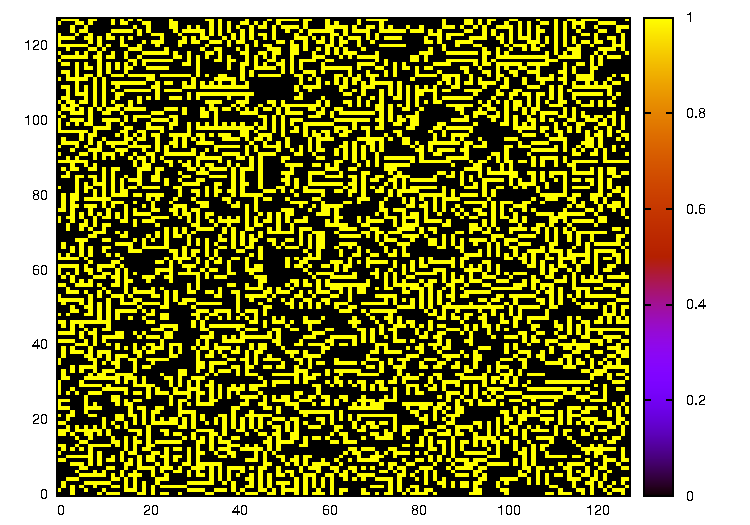
\includegraphics{plts/gol-128-100-0-16.pdf}
\caption{Final state for 128x128 universe, 100 ticks and threshold 0\%}
\label{fig:0}
\end{figure}
\begin{figure}[t]
\centering
   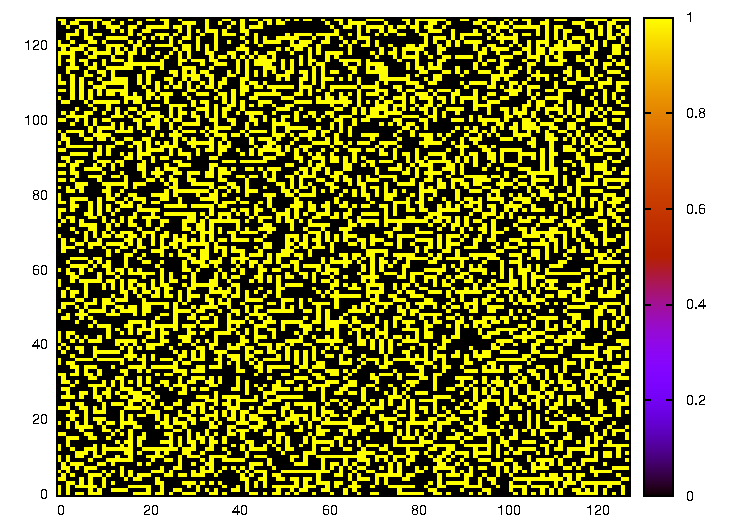
\includegraphics{plts/gol-128-100-25-16.pdf}
\caption{Final state for 128x128 universe, 100 ticks and threshold 25\%}
\label{fig:25}
\end{figure}
\begin{figure}[t]
\centering
   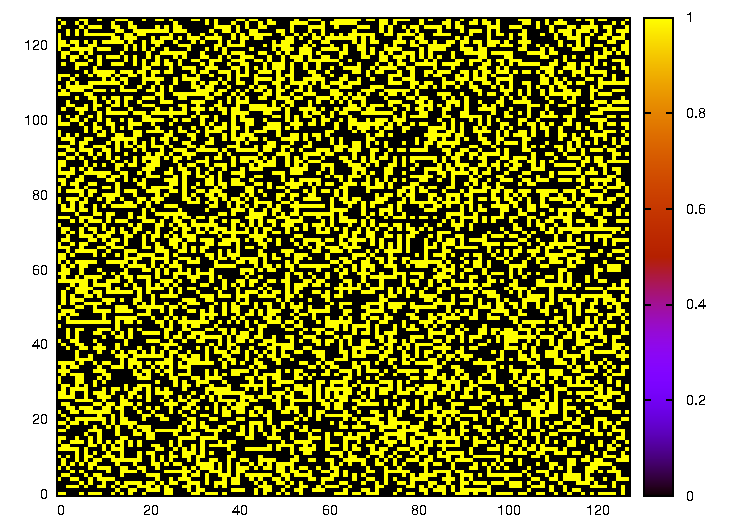
\includegraphics{plts/gol-128-100-50-16.pdf}
\caption{Final state for 128x128 universe, 100 ticks and threshold 50\%}
\label{fig:50}
\end{figure}
\begin{figure}[t]
\centering
   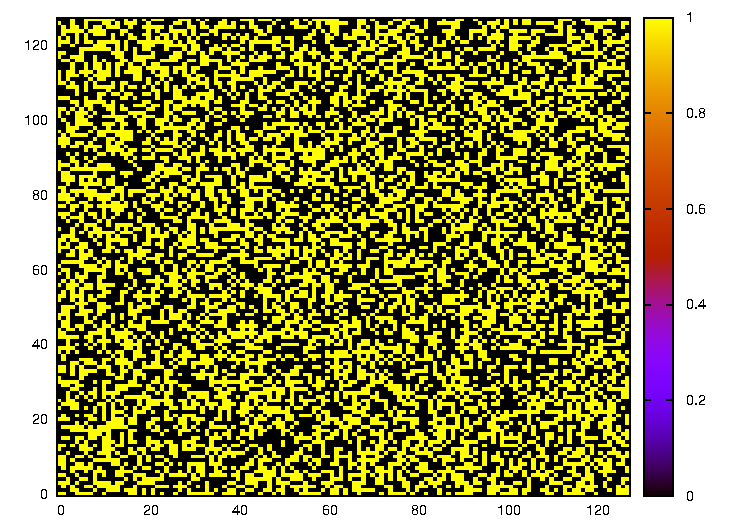
\includegraphics{plts/gol-128-100-75-16.pdf}
\caption{Final state for 128x128 universe, 100 ticks and threshold 75\%}
\label{fig:75}
\end{figure}
\begin{figure}[t]
\centering
   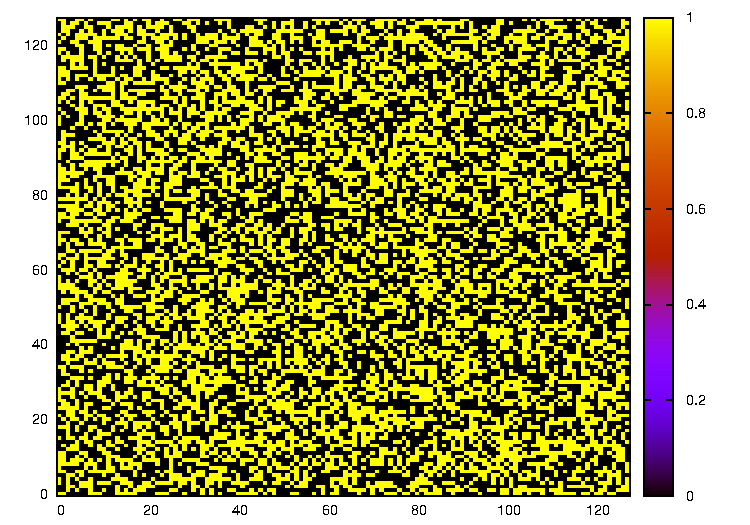
\includegraphics{plts/gol-128-100-90-16.pdf}
\caption{Final state for 128x128 universe, 100 ticks and threshold 90\%}
\label{fig:90}
\end{figure}
\begin{figure}[t]
\centering
   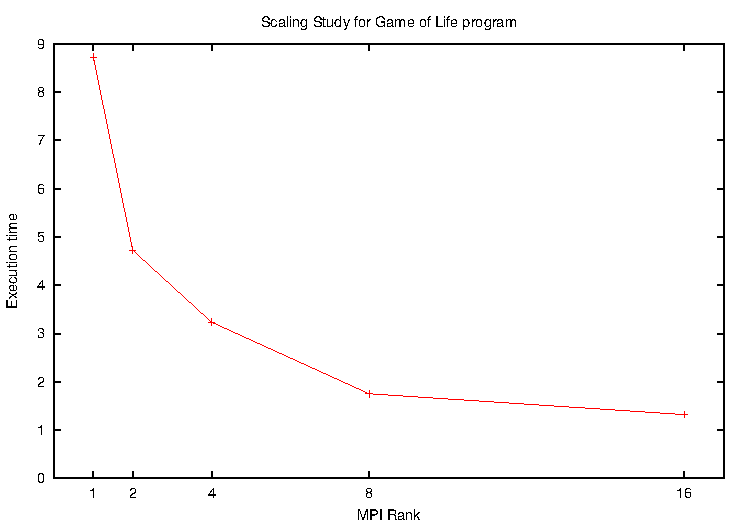
\includegraphics{plts/scaling.pdf}
\caption{Scaling study performed for 1024x1024 cell universe, 100 ticks, and 25\% threshold}
\label{fig:scaling}
\end{figure}






%\bibliography{main}

%\bibliographystyle{abbrv}
\end{document}
